\documentclass[DeseNET_Sebastien_Deriaz]{subfiles}



\begin{document}
\section{Fonctionnement}
La station de base (que l'on programme) doit être capable, lorsqu'elle reçoit une trame spéciale (beacon), de renvoyer les données qu'elle a collecté. Ces données sont :
\begin{enumerate}
\item Événements (par exemple un mouvement sur le joystick)
\item État mesuré (par exemple l'accéléromètre embarqué)
\end{enumerate}
\begin{figure}[H]
\centering
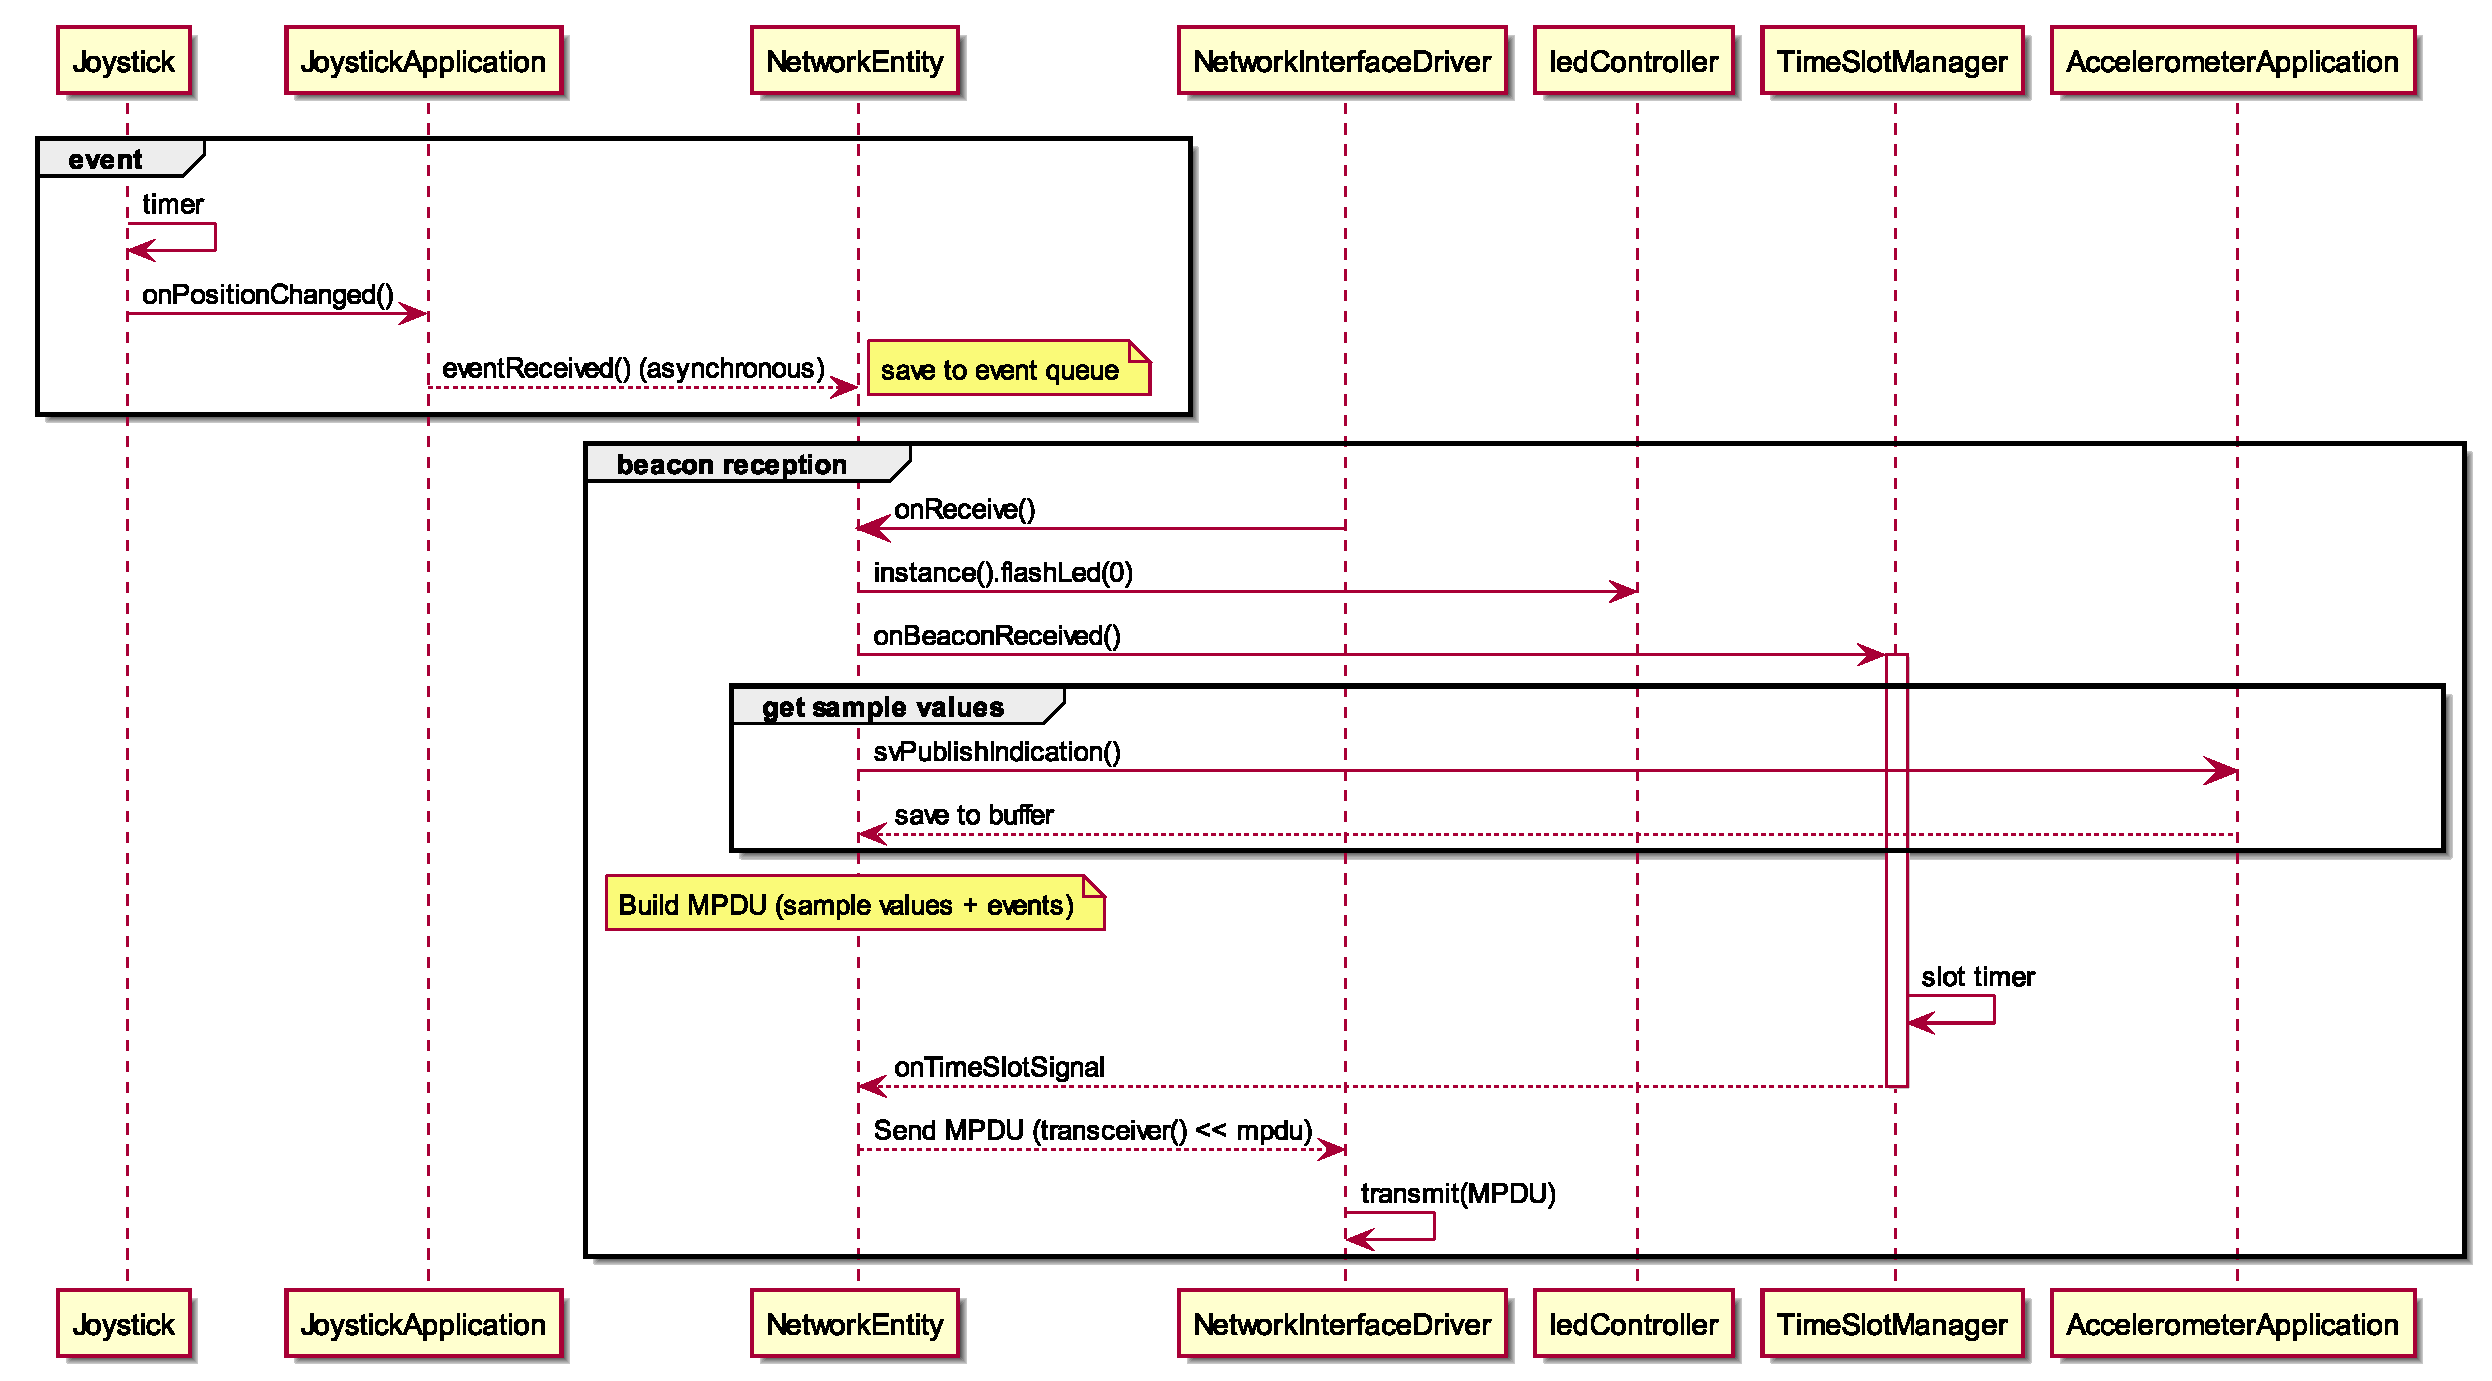
\includegraphics[width=0.9\textwidth]{out/sequence_beacon.eps}
\caption{Diagramme de séquence}
\end{figure}
\pagebreak
\subsection{Classe \texttt{MPDU}}
Le classe MPDU permet de construire une frame contenant des données d'événements et/ou des "sampled values" (valeurs mesurées demandées par la station de base).
\begin{figure}[H]
\centering
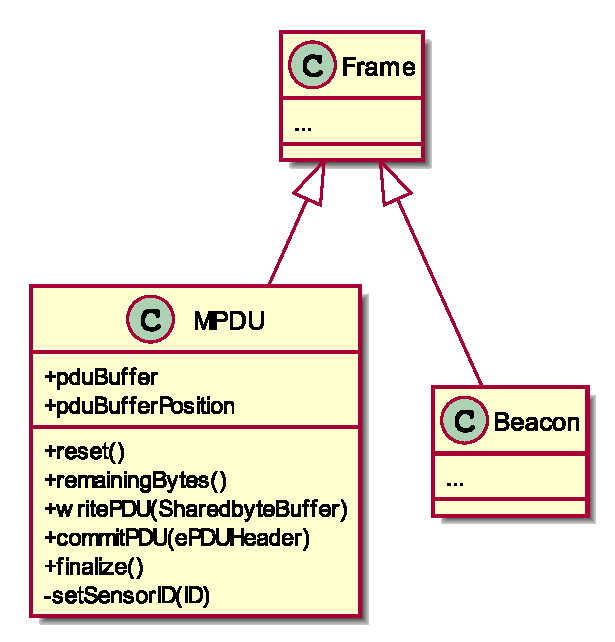
\includegraphics[scale=0.5]{out/MPDU.eps}
\caption{Classe \texttt{MPDU}}
\end{figure}
Les informations des classes \verb!Beacon! et \verb!Frame! n'ont pas été notées car elles n'ont pas été modifiées.\\
\subsubsection{Description des méthodes}
\begin{enumerate}
\item \verb!pduBuffer! : \verb!SharedByteBuffer! qui permet l'écriture sur le buffer du MPDU. Le début de ce buffer avance continuellement à mesure que de nouvelles données sont écrites dans le MPDU.
\item \verb!pduBufferPosition! : Position actuelle du \verb!pduBuffer! à l'intérieur du "vrai" buffer. Ceci permet à une application d'écrire dans la frame au bon endroit
\begin{figure}[H]
\centering
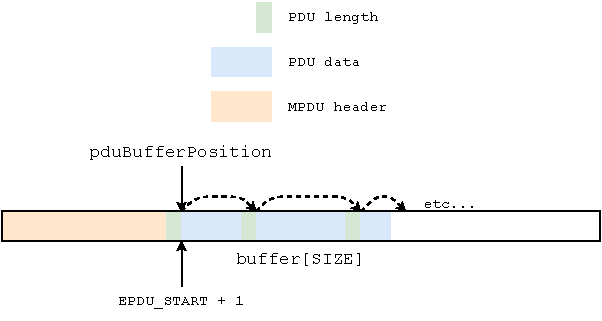
\includegraphics[scale=1]{drwg_0.pdf}
\end{figure}
\item \verb!reset()! permet de réinitialiser le MPDU (position dans le buffer, données, etc...)
\item \verb!remainingBytes()! : donne une information sur la place restante pour écrire les données des applications
\item \verb!writePDU()! : Écrire des données dans le buffer (à la position donnée par \verb!pduBufferPosiiton!
\item \verb!finalize()! : Conditionne le MPDU pour l'envoi final (headers)
\item \verb!setSensorID()! : Enregistre le numéro de slot dans le MPDU (pour l'écrire du header MPDU)
\end{enumerate}
La création d'un MPDU (pour l'envoi à la station de base) se fait de la manière suivante :
\begin{enumerate}
\item Reset
\item Ajout des sample values (accéléromètre)
\item Ajout des événements (jusqu'à ce qu'il n'y en ait plus ou que le buffer soit plein). Effectuer un "commit" après chaque événement
\item Finalisation
\end{enumerate}
Une fois qu'un MPDU est prêt, il est envoyé au moment où le temps du slot est atteint (slot timer).\\
\subsubsection{svPDU}
Pour stocker les données mesurées, on commence par vérifier si le groupe de mesures (\verb!svGroup!) est demandé dans le beacon.\\
Si c'est le cas, on appelle la méthode \verb!svPublishIndication! de chaque application en passant un buffer. L'application va écrire les données dans ce buffer puis retourner le nombre de bytes écris. On appelle ensuite la méthode \verb!commit! du MPDU qui va créer le header pour ces données. On recommence cette séquence pour chaque svGroup.
\subsubsection{evPDU}
Une fois que tous les svPDU sont stockés, on rempli le MPDU avec des evPDU (tant qu'il y en a ou jusqu'à ce que le MPDU soit plein). Pour cela on va lire une liste des événements (\verb!eventsQueue!) et ajouter chaque élément dans l'ordre.\\
Si le MPDU est plein, on supprime les événements restants (il est possible de perdre des changements d'état sur le joystick).
\subsubsection{Envoi}
Lorsque le timeslot est atteint (Temps du slot $\times$ numéro de slot en millisecondes), on envoie le MPDU à la station de base.\\
On utilise la fonction \verb!onTimeSlotSignal! en vérifiant que le signal émis est \verb!OWN_SLOT_START!. Si cette vérification n'est pas faite, le MPDU sera envoyé plusieurs fois (lors d'autres signaux qui ne correspondent pas).
\pagebreak
\subsection{Classe \texttt{JoystickApplication}}
La classe \verb!JoystickApplication! a été copiée à partir de la classe \verb!AccelerometerApplication!
\begin{figure}[H]
\centering
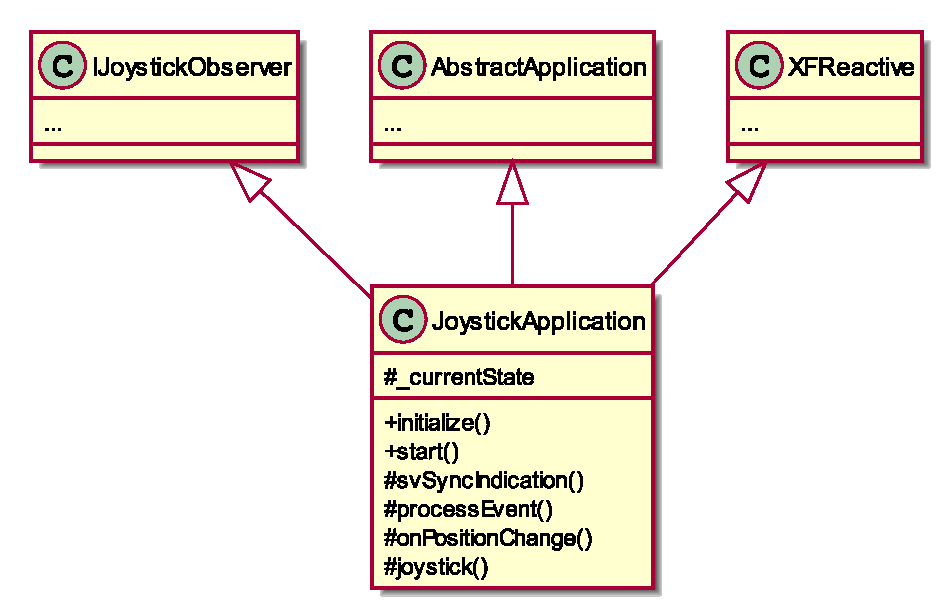
\includegraphics[scale=0.5]{out/JoystickApplication.eps}
\caption{Classe \texttt{JoystickApplication}}
\end{figure}
\begin{enumerate}
\item \verb!_currentState! : état actuel de la machine d'état
\item \verb!initialize()! : Initialisation de l'application (inscription vers le \verb!networkentity! avec le bon numéro de groupe)
\item \verb!start()! : démarrage de la machine d'état
\item \verb!svSyncIndication()! : méthode appelée lorsque le beacon est reçu (pour la synchronisation des applications)
\item \verb!processEvent()! : traitement des événements de la machine d'état
\item \verb!onPositionChange()! : méthode appelée lorsqu'un mouvement est détecté sur le joystick (vient de \verb!IJoystick!)
\item \verb!joystick()! méthode permettant d'obtenir le singleton \verb!joystick! (depuis la \verb!Factory!)
\end{enumerate}
\begin{figure}[H]
\centering
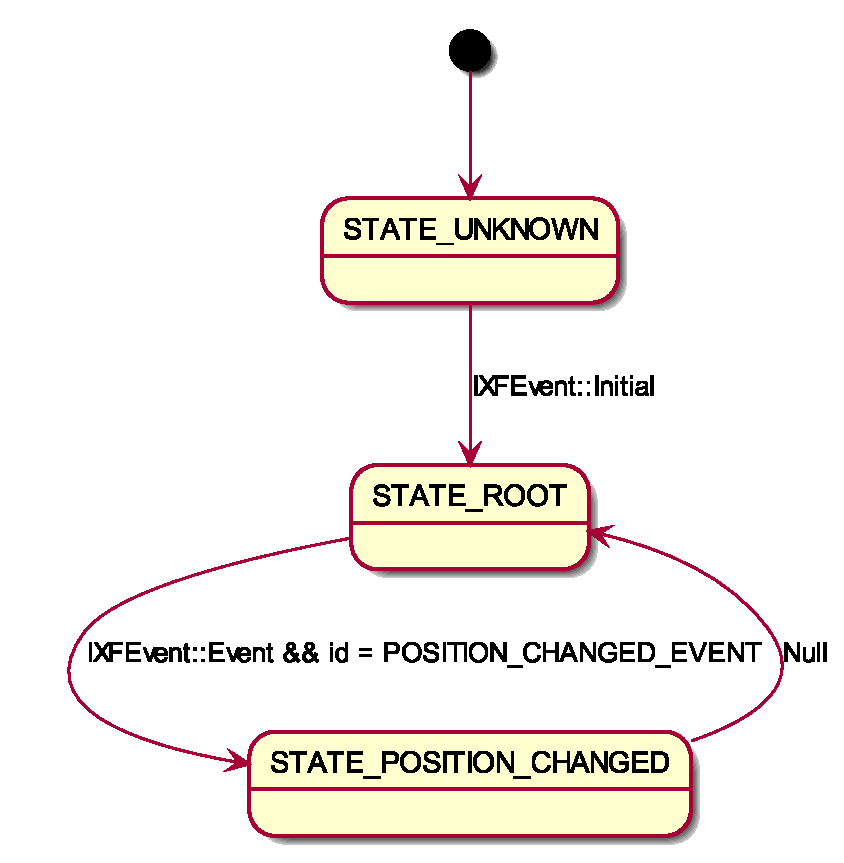
\includegraphics[scale=0.5]{out/SM.eps}
\caption{Machine d'état de \texttt{JoystickApplication}}
\end{figure}
\end{document}